\section{Proposta}

Este trabalho propõe a criação de um protótipo destinado a gerar um mapa de forma procedural, cujo contorno é selecionado a partir de uma imagem processada por um modelo de segmentação panóptica \footnote{No resultado apenas será identificado os pixeis de classes contidas nos conjuntos de dados escolhidos, e todos citados no capítulo 2 são de contexto urbano}. O mapa resultante replicará o contorno da seleção em duas dimensões e três dimensões.

A \cref{fig:etapas_proposta} apresenta os passos dessa abordagem, onde a imagem a representa a entrada para o processo de segmentação panóptica, e a imagem b é o resultado desse processo. Utilizou-se o modelo de segmentação panóptica EfficientPS criado por \citeonline{mohan2020efficientps}, uma solução eficiente para segmentação panóptica e de acordo com \citeonline{datasetResults} possui a melhor classificação da métrica de qualidade panóptica definida por \citeonline{kirillov2019panoptic} para classificar pessoas, o que é importante em um contexto atual segundo \citeonline{dp_semantic_segmantation}, e pode ser encontrado no repositório dos próprios autores \citeonline{mohan2020efficientps} disponível na internet. Após a segmentação da imagem, o usuário terá a capacidade de selecionar um contorno com as técnicas de selecionar por cor e por preenchimento de inundação de acordo com \citeonline{OpenCVInRange} e \citeonline{OpenCVFloodFill}, respectivamente. Além disso decidiu-se criar mais duas opções para segmentação devido a limitação dos conjuntos de dados para segmentação panóptica, de acordo com \citeonline{v7labs2022panoptic} os conjuntos são de contexto urbano o que limita o número de classes de objetos, logo adicionar a seleção por cor e por preenchimento de inundação aumentará a gama de utilização, possibilitando por exemplo selecionar um desenho feito em uma folha sulfite.
O resultando da seleção será uma máscara binária de acordo com \citeonline{Embarcados} é uma maneira de isolar um objeto na imagem, conforme ilustrado na imagem c, que representa a escolha do segmento, nesse exemplo o carro amarelo da imagem b. Subsequentemente, um mapa procedural, que segundo \citeonline{yannakakis2018artificial} são métodos e automações que geram mapas, será gerado com o contorno escolhido, conforme evidenciado na imagem d. Essa representação incluirá uma sobreposição do contorno do veículo, meramente para ilustrar que a ilha gerada terá um contorno semelhante. As cores na representação indicam o oceano (azul), a floresta (verde) e as montanhas (cinza). Além disso, será automatizado para atualizar o relevo de um mapa em três dimensões.

% footnote?
%
% Após a segmentação da imagem — como ilustra a \cref{fig:segmantations_2} — o usuário poderá selecionar uma das áreas coloridas da imagem que será utilizada para gerar a ilha.

% Em seguida será criado um diagrama de Voronoi (pode ser observado na \cref{fig:diagrama_voronoi}), esse diagrama será utilizado para marcar a localização da ilha, assim gerando o mapa e os biomas a partir da atribuição de propriedades para cada ponto, polígono e reta do diagrama.

% O resultado esperado pode ser contemplado na \cref{fig:resultado_geracao}, onde o azul representa o oceano, o verde retrata a floresta e o cinza caracteriza uma montanha.


\begin{figure}[!ht]
	\centering
    \caption{Etapas da proposta}
	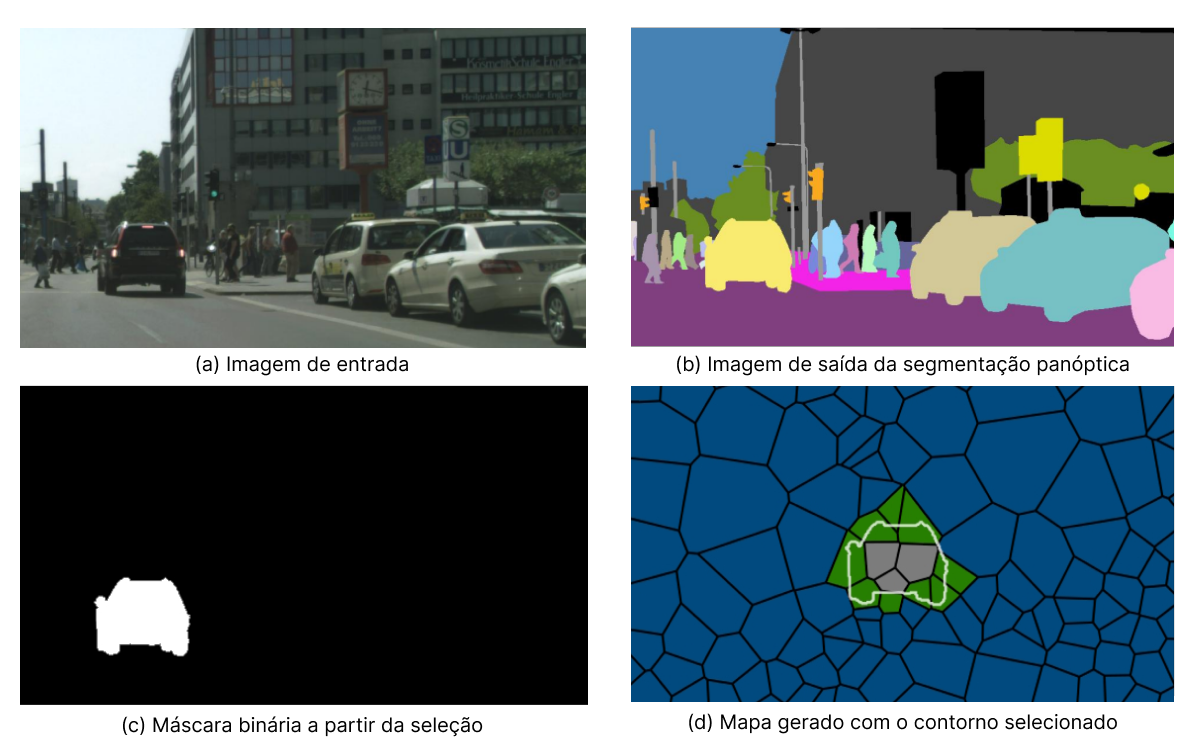
\includegraphics[width=0.9\textwidth]{figures/etapas_proposta.png}
    \legend{Fonte: \citeonline{kirillov2019panoptic} e autoria própria}
	\label{fig:etapas_proposta}
\end{figure}


% \begin{figure}[!ht]
% 	\centering
%     \caption{Imagem de entrada para rede neural.}
% 	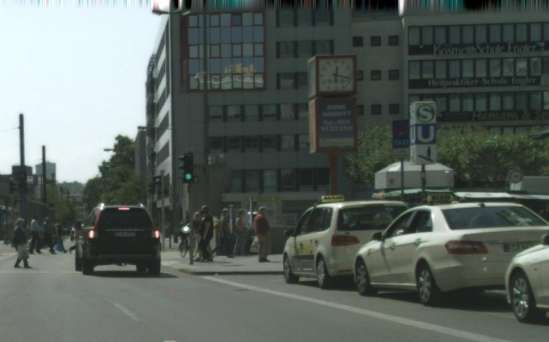
\includegraphics[width=0.6\textwidth]{figures/segmantations_1.png}
%     \legend{Fonte: \citeonline{kirillov2019panoptic}}
% 	\label{fig:segmantations_1}
% \end{figure}

% \begin{figure}[!ht]
% 	\centering
%     \caption{Imagem saída de um modelo de segmentação panóptica.}
% 	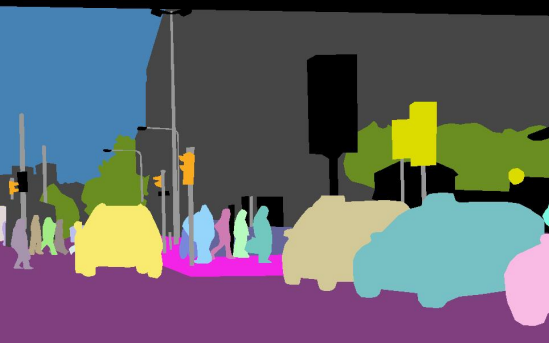
\includegraphics[width=0.6\textwidth]{figures/segmantations_2.png}
%     \legend{Fonte: \citeonline{kirillov2019panoptic}}
% 	\label{fig:segmantations_2}
% \end{figure}

% \begin{figure}[!ht]
% 	\centering
%     \caption{Ilha gerada a partir da segmentação panóptica e aplicando um filtro com o diagrama de Voronoi, azul representa oceano, verde floresta, cinza montanhas.}
% 	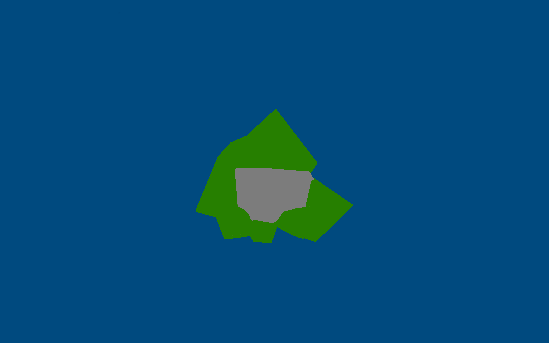
\includegraphics[width=0.6\textwidth]{figures/segmantations_pnl.png}
%     \legend{Fonte: Criação própria}
% 	\label{fig:resultado_geracao}
% \end{figure}

